
\documentclass[calculator,steamtables,refrigeranttables,psychrometricchart,datasheet,solutions]{exam}
%\documentclass[calculator,datasheet]{exam}
%\documentclass[calculator,datasheet,solutions]{exam}


% The full list of class options are
% calculator : Allows approved calculator use.
% datasheet : Adds a note that data sheet are attached to the exam.
% handbook : Allows the use of the engineering handbook.
% resit : Adds the resit markings to the paper.
% sample : Adds conspicuous SAMPLE markings to the paper
% solutions : Uses the contents of \solution commands (and \solmarks) to generate a solution file

\usepackage{pdfpages}
\usepackage{lscape,comment}

\coursecode{EG5597}%
\coursetitle{Advanced Chemical Engineering}%
\examtime{00.00--00.00}%
\examdate{00}{08}{2014}%
\examformat{Candidates must attempt \textit{all} questions.}

\newcommand{\frc}{\displaystyle\frac}
\newcommand{\br}[1]{\!\left( #1 \right)}
\newcommand{\abs}[1]{\left| #1 \right|}
\newcommand{\fracd}[2]{\frac{\mathrm{d} #1}{\mathrm{d} #2}}
\newcommand{\fracp}[2]{\frac{\partial #1}{\partial #2}}
\renewcommand{\d}[1]{\mathrm{d} #1 }
\newcommand{\Ma}{\mathrm{M\!a}}



\begin{document}

%%%
%%% Question 01 
%%%
\begin{question} %\vspace{-2\baselineskip}

%
%%%
In fluid mechanics problems, we often deal with an open, bounded spatial region $\Omega$ and on the boundary $\Gamma=\partial\Omega$. A chemical species with concentration $\mathcal{C}\left(\underline{x},t\right)$ is transported within a bounded region (i.e., in a stirred tank) and satisfies appropriate boundary conditions. Assume that $\underline{\bf{n}}$ is the outward normal vector on the boundary $\left(\underline{x}\in\Gamma\right)$ with inflow boundary $\underline{n}.\underline{u} < 0$ (where $\underline{u}$ is the velocity vector field). In order design an stirred tank with optimal mixing performance, an engineering team will need to solve an advection-diffusion problem with a commercial CFD.
\begin{enumerate}[(i)]
%%% 
%%% Question 1
%%%
\item Define the 3 types of boundary conditions used to solve PDEs.~\marks{6}
\solution{%%% 
\begin{enumerate}[(a)]
\item In Dirichlet BC, one prescribes the value of a variable at the boundary,~\solmarks{2/6}
  \begin{displaymath}
    \mathcal{C}=\mathcal{C}_{D}\;\;\;\;\text{ on }\Gamma_{D}
  \end{displaymath} 
where $\mathcal{C}_{D}$ is a constant.
\item In Newmann BC, one prescribes the gradient normal to the boundary of a variable at the boundary,~\solmarks{2/6}
  \begin{displaymath}
    \underline{n} . \nabla{\mathcal{C}} = \mathcal{C}_{N} \;\;\;\;\text{ on } \Gamma_{N}
  \end{displaymath}
where $\mathcal{C}_{N}$ is a constant.
\item In mixed (or Robin) BC, a function of the form~\solmarks{2/6}
\begin{displaymath}
\underline{n}\left(\underline{u}\mathcal{C}-\mathcal{D}\nabla\mathcal{C}\right)=\mathcal{C}_{R}\;\;\;\;\text{ on } \Gamma_{R}
\end{displaymath}
where $\mathcal{C}_{R}$ and $\mathcal{D}$ are constants.
\end{enumerate}
}

%%%
%%% Question 2
%%%
\item Define finite difference methods.~\marks{2}
\solution{%%%
Finite difference method consists in approximating the differential operator by replacing the derivatives in the equation using differential quotients. The spatial and temporal domains are subdivided and approximations of the solution are obtained.  The error (i.e., discretisation or truncation error) between the actual numerical solution and the exact solution is determined by the error that is committed by going from a differential operator to a difference operator.~\solmarks{2/2}
}

%%%
%%% Question 3
%%%
\item Chemical species are advected (in 1D) at velocity $u_{x}=0.50$ m/s with time-step size $\left(\Delta t\right)$ of $3$s through $60$ m. Discretising the transport equation in space and time, the concentration can be calculated, using FDM, as~\marks{10}
\begin{displaymath}
\mathcal{C}_{i}^{j+1}=\mathcal{C}_{i}^{j} - \frac{u\Delta t}{\Delta x }\left(\mathcal{C}_{i+1}^{j}-\mathcal{C}_{i}^{j}\right)
\end{displaymath}
where $i\in\left\{1,2,...,N_{x}\right\}$ and $j\in\left\{0,1,...,k\right\}$ are spatial- and time-increment indexes, respectively. Assume:
\begin{itemize}
\item The domain is divided into $N_{x}=4$ nodes;
\item Initial condition is given by,
\[
\mathcal{C}\left(x,t=0\right)=
\left\{\begin{array}{l l}
0.075 + e^{-0.01\left(x-45\right)^{2}} & \text{for } 20 \le x \le 40 \\
0.0 & \text{elsewhere.}
\end{array}\right.\]
\item The {\it ghost-node}: $x_{N_{x}+1}=x_{N_{x}}$
\end{itemize}
Calculate $\mathcal{C}_{i}^{1}$ (i.e., at $j = 1$ -- a-d).\\
%\begin{center}
\hbox{\hspace{4.cm}\begin{tabular}{||c | c c c c ||}
\hline\hline
{\bf i} & 1   & 2    & 3   &  4   \\
\hline\hline
$x_{1}$ &   &   &  &  \\
$\mathcal{C}_{i}^{0}$ &  & &  &  \\
$\mathcal{C}_{i}^{1}$ & (a) & (b) & (c) & (d) \\
\hline\hline
\end{tabular}}
%\end{center}
\solution{%%%
First we need to calculate $\Delta x$~\solmarks{2/10}
\begin{displaymath}
\Delta x = \frac{X_{f}-X_{0}}{N_{x} - 1} = \frac{60 - 0}{4 - 1 } = 20.0
\end{displaymath}
Solving for concentration at time step $j=0$ is by solving the equation
\begin{eqnarray}
\mathcal{C}_{i}^{j+1}=\mathcal{C}_{i}^{j} - \frac{u\Delta t}{\Delta x }\left(\mathcal{C}_{i+1}^{j}-\mathcal{C}_{i}^{j}\right) \nonumber \\
\mathcal{C}_{1}^{1}=\mathcal{C}_{1}^{0} - \frac{0.5 \times 3.0}{20.0} \left(\mathcal{C}_{2}^{0}-\mathcal{C}_{1}^{0}\right) \nonumber \\
\mathcal{C}_{2}^{1}=\mathcal{C}_{2}^{0} - \frac{0.5 \times 3.0}{20.0} \left(\mathcal{C}_{3}^{0}-\mathcal{C}_{2}^{0}\right) \nonumber \\
\mathcal{C}_{3}^{1}=\mathcal{C}_{3}^{0} - \frac{0.5 \times 3.0}{20.0} \left(\mathcal{C}_{4}^{0}-\mathcal{C}_{3}^{0}\right) \nonumber
\end{eqnarray}
The table becomes:\\~\solmarks{8/10}
\begin{center}
%\hbox{\hspace{2.cm}
\begin{tabular}{||c | c c c c ||}
\hline\hline
{\bf i} & 1   & 2    & 3    &  4   \\
\hline\hline
$x_{1}$ & 0    &  20  & 40   & 60   \\
$\mathcal{C}_{i}^{0}$ &  0.00 & 0.0769  &  0.85380  & 0.00  \\
$\mathcal{C}_{i}^{1}$ & (a) 0.00 & (b) 0.18665 & (c) 0.91783 & (d) 0.00 \\
\hline\hline
\end{tabular}%}
\end{center}
}

\item Solving the transport equation with finite volume method resulted in the following linear system -- $\mathcal{A}x=b$, or in matricial form,
\[
\begin{pmatrix} 3 & 1 & 1 \\ 1 & 2 & 0 \\ 1 & 0.5 & 2 \end{pmatrix}
\begin{pmatrix} x_{1} \\ x_{2} \\ x_{3} \end{pmatrix} =
\begin{pmatrix} 4.5 \\ 2.0 \\ 2.45 \end{pmatrix}
\]
In order to solve this system, the team used a relaxation iterative method:
\begin{displaymath}
x_{i}^{(k+1)} = \left(1 - \omega\right) x_{i}^{(k)} + \omega \left[ \frac{b_{i}}{a_{ii}} - \sum\limits_{j=1}^{i-1} \frac{a_{ij}}{a_{ii}}x_{j}^{(k+1)} - \sum\limits_{j=i+1}^{n} \frac{a_{ij}}{a_{ii}}x_{j}^{(k)}\right]
\end{displaymath}
with $\omega=1.08$. Calculate $x^{1}$ with $x^{0}=\left(\;1 \; 1 \; 1\;\right)^{T}$.~\marks{7}
\solution{%%%
The solution vector $x^{1}=\left( 0.8199 \;\; 0.5572 \;\; 0.6498\right)^{T}$.~\solmarks{7/7}
}

\end{enumerate}

\end{question}


\clearpage

\paperend

%\begin{comment}
%\begin{landscape}
%\begin{center}
%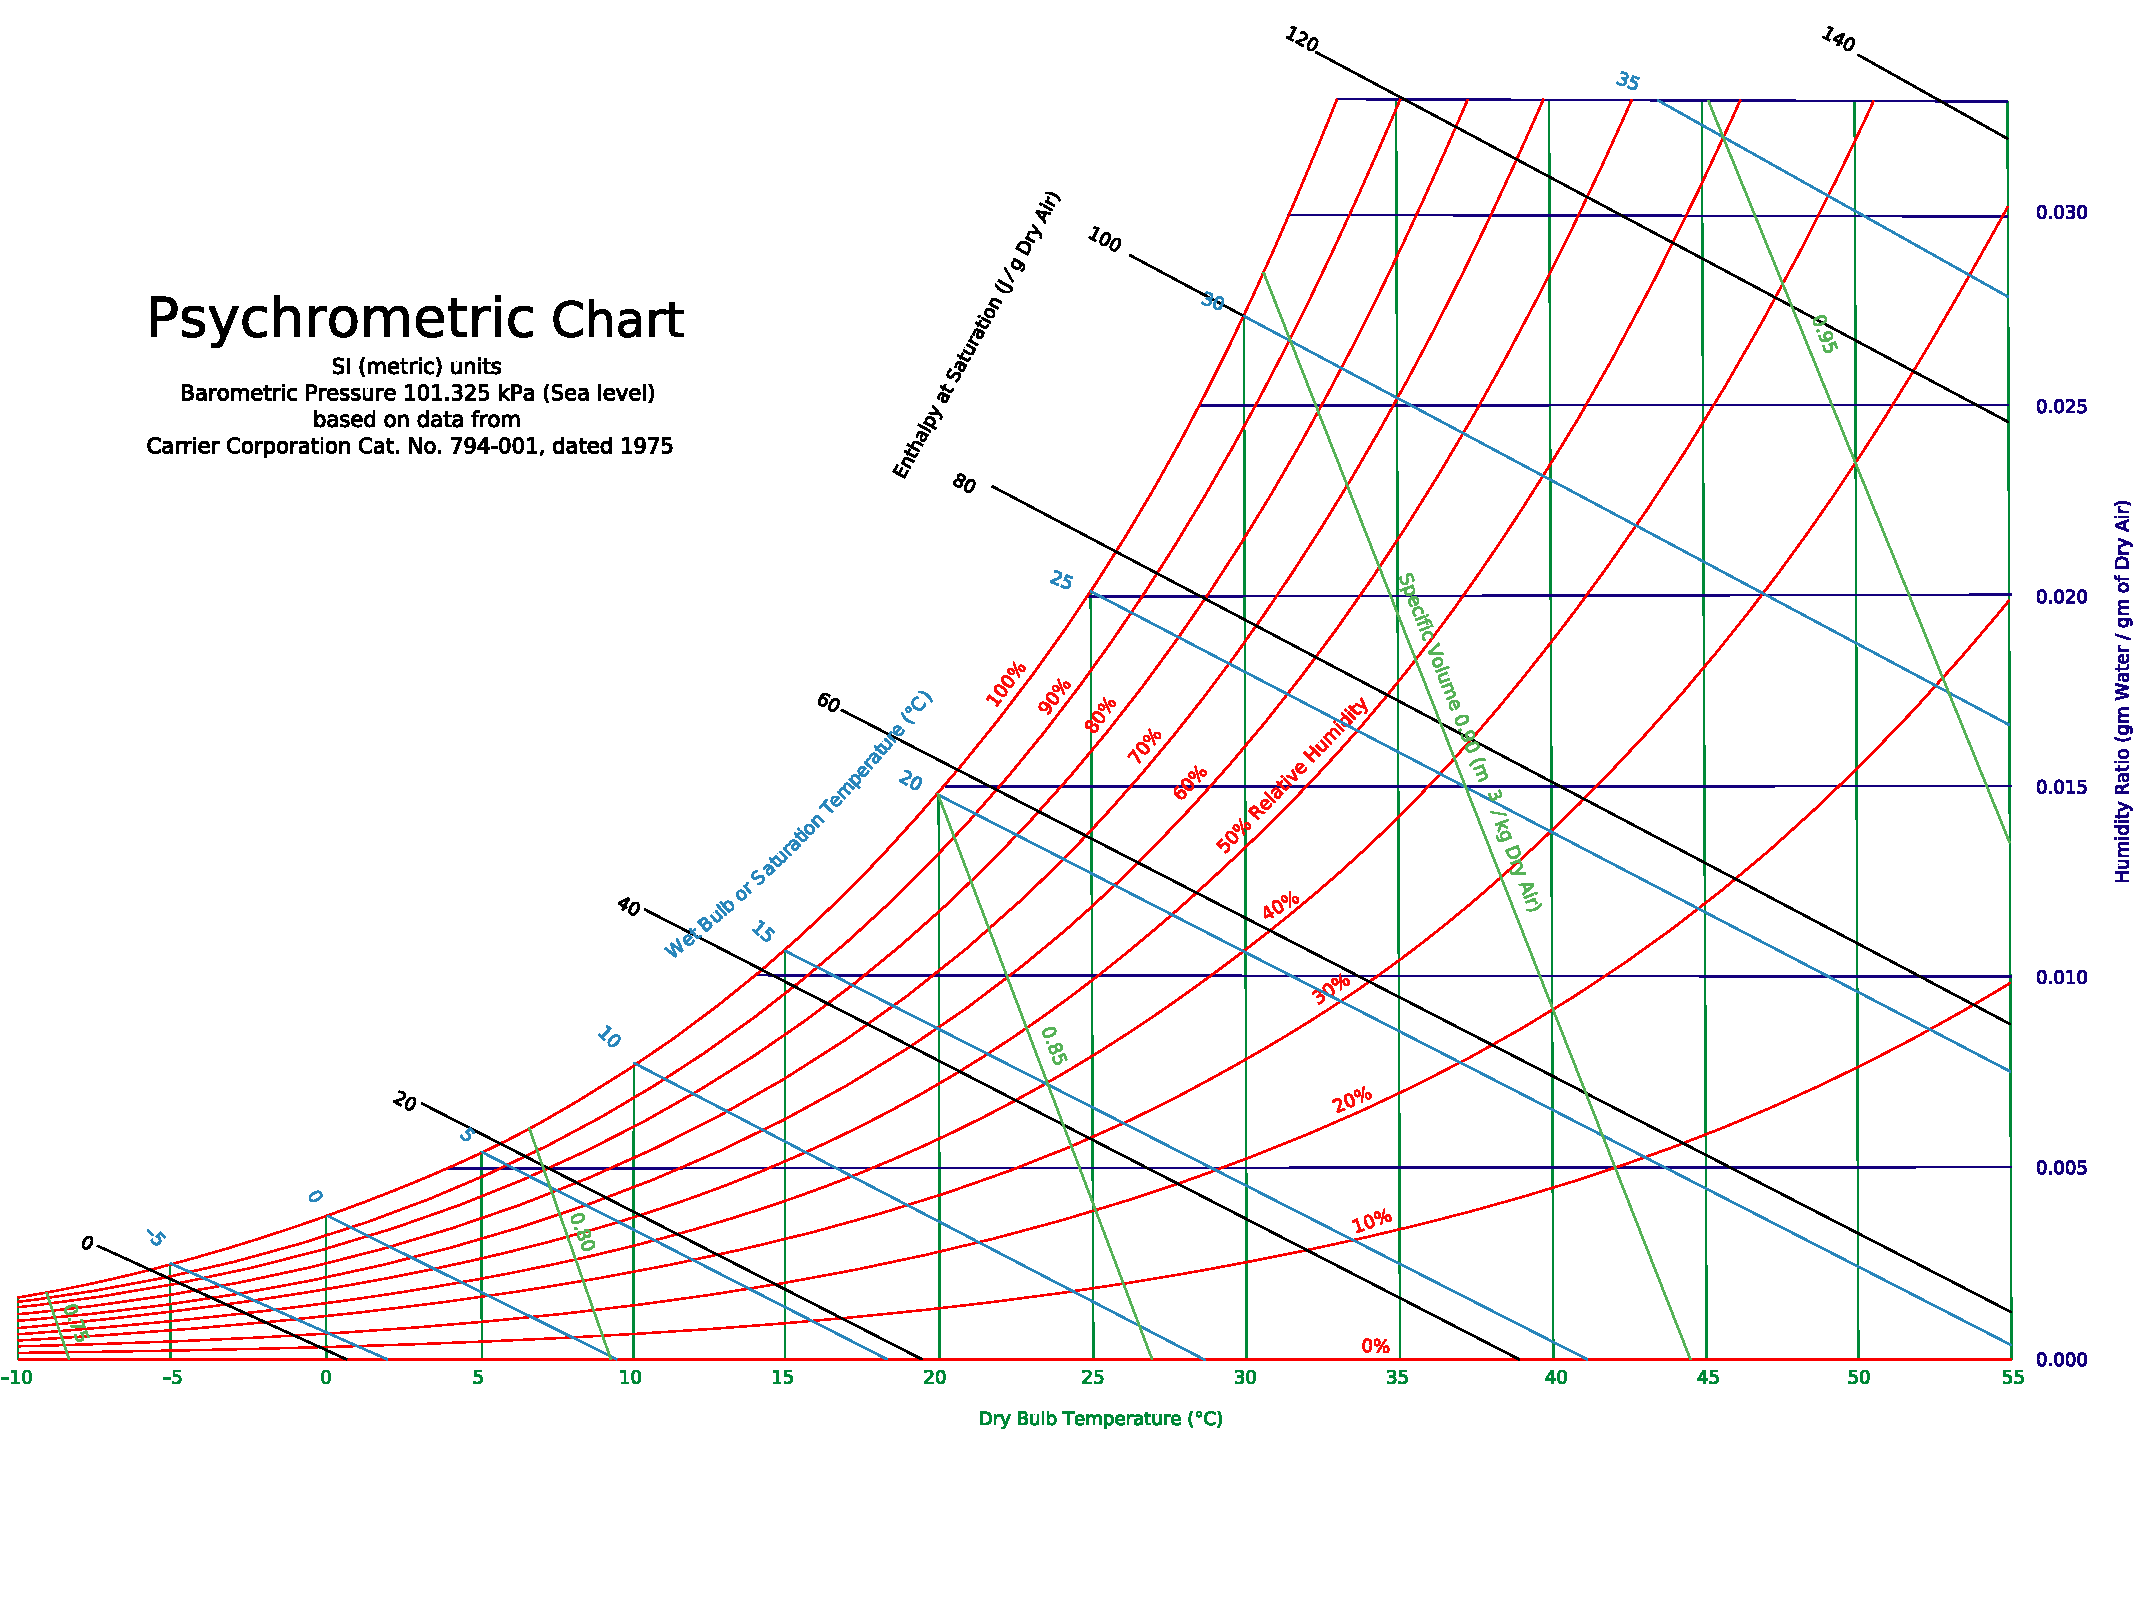
\includegraphics[width=1.5\textwidth]{PsychrometricChart}
%\end{center}
%{
%  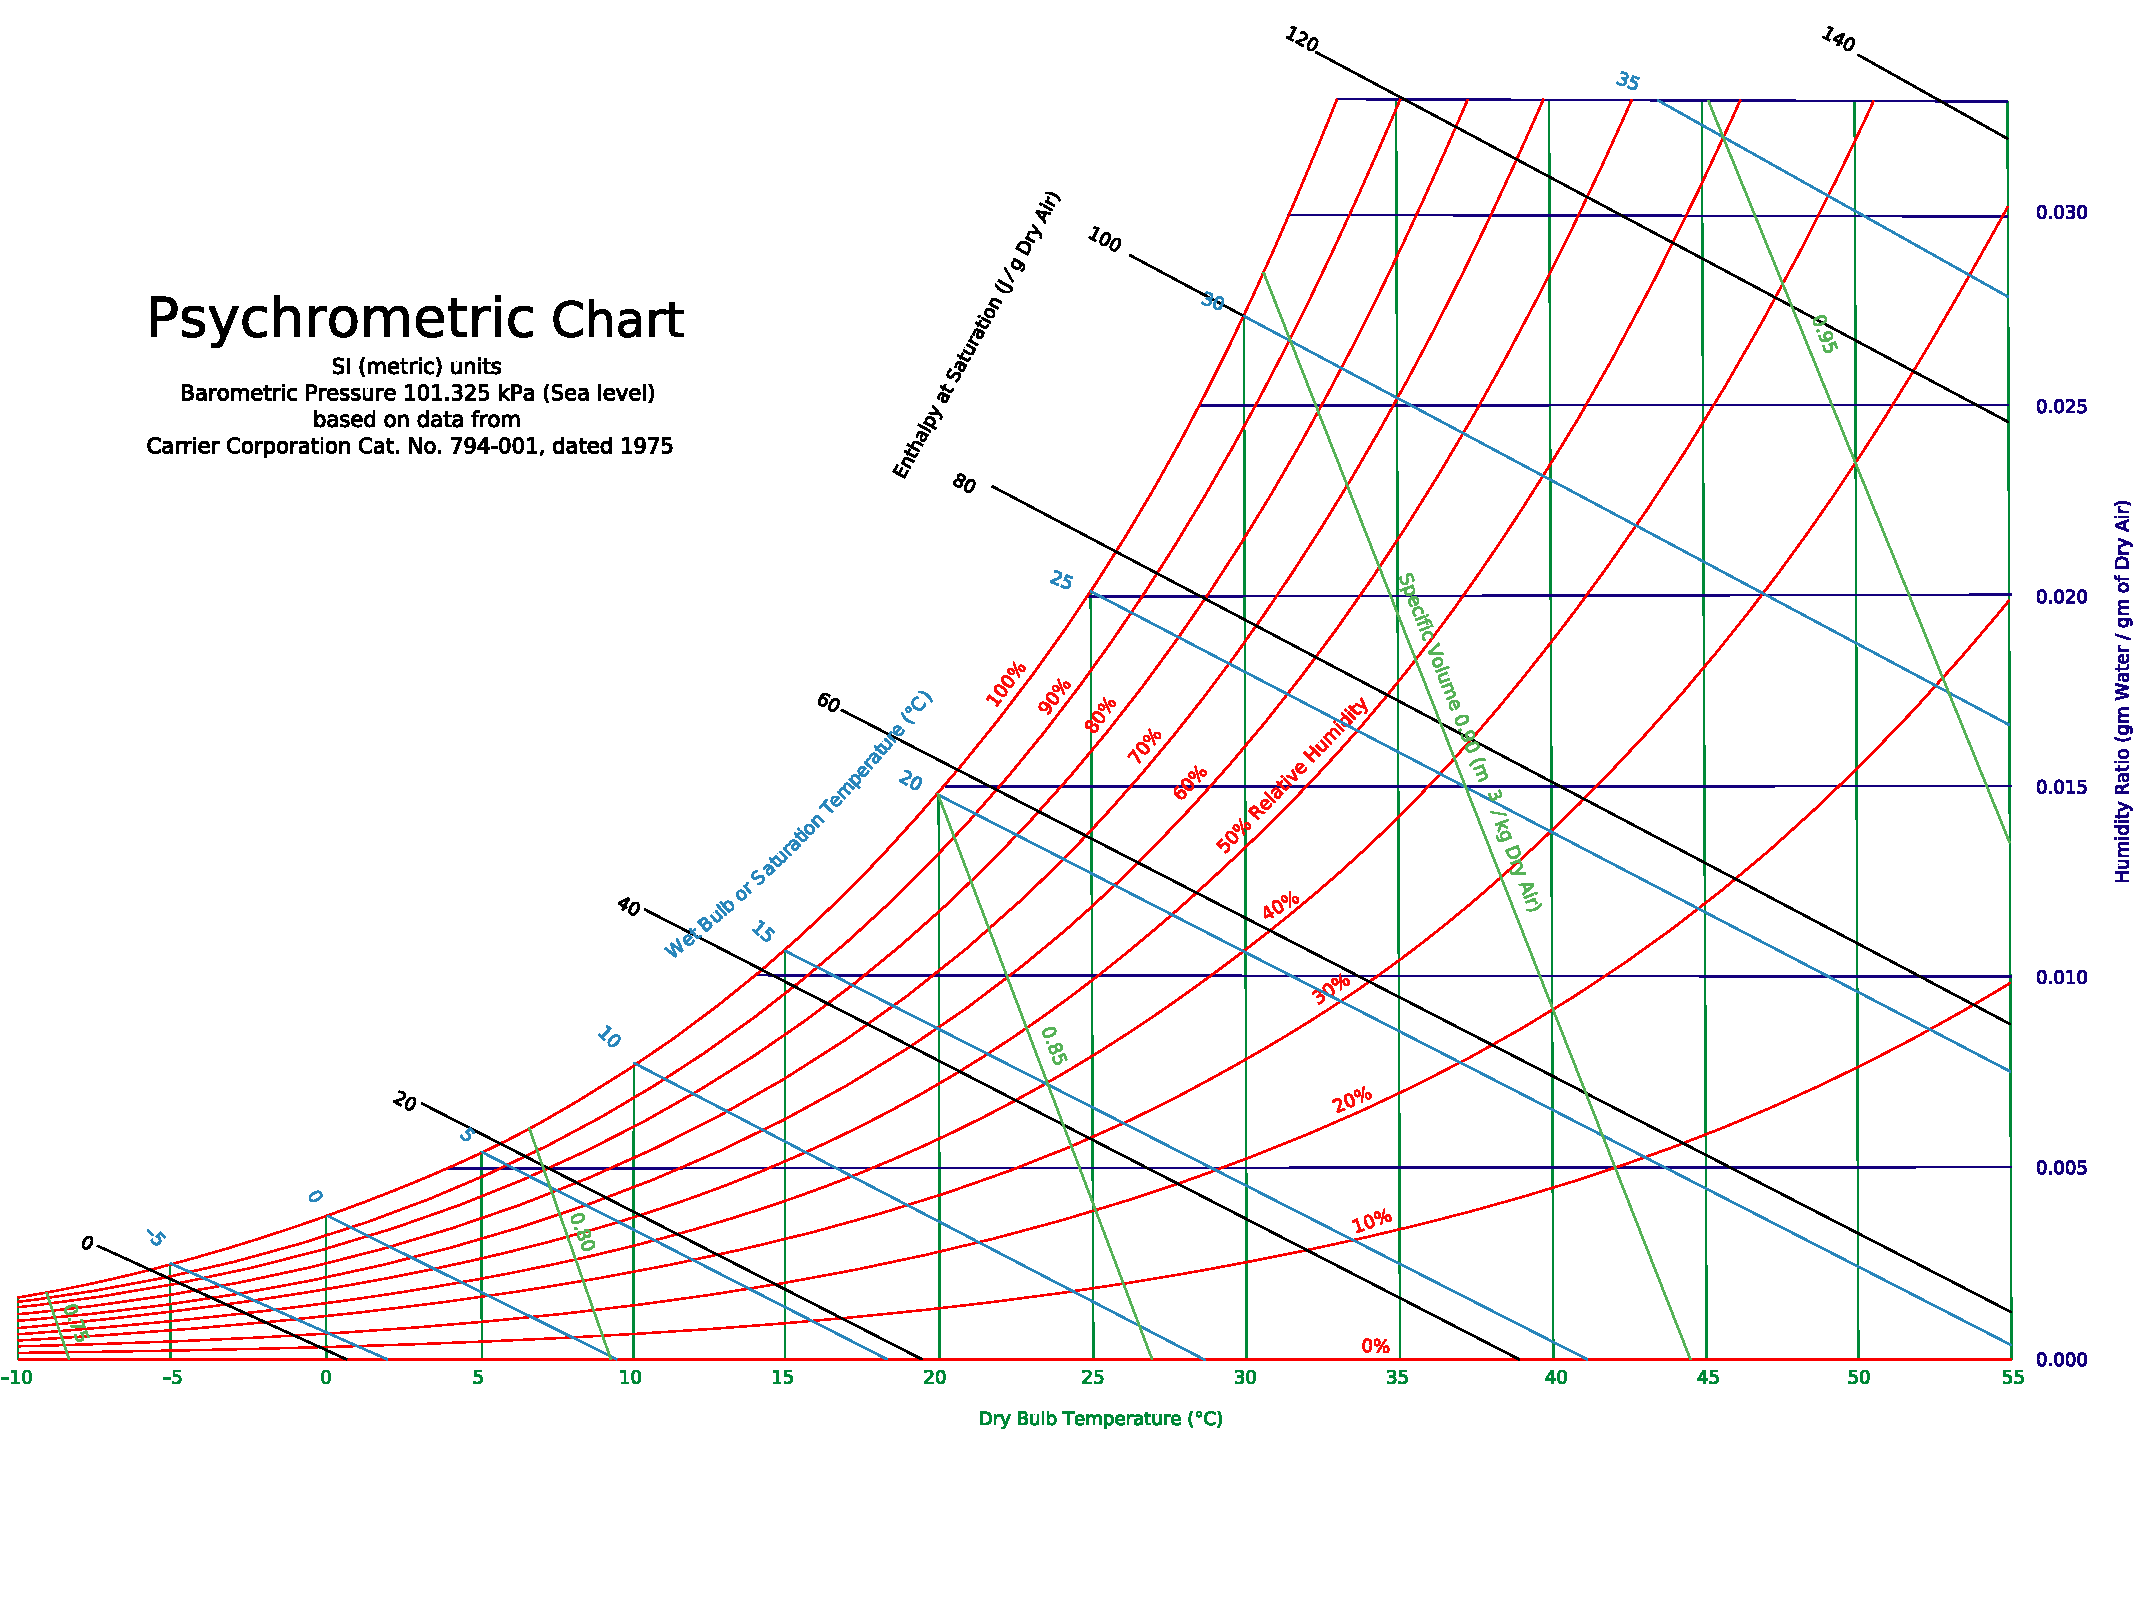
\includepdf[pages=-,fitpaper]{PsychrometricChart}
%  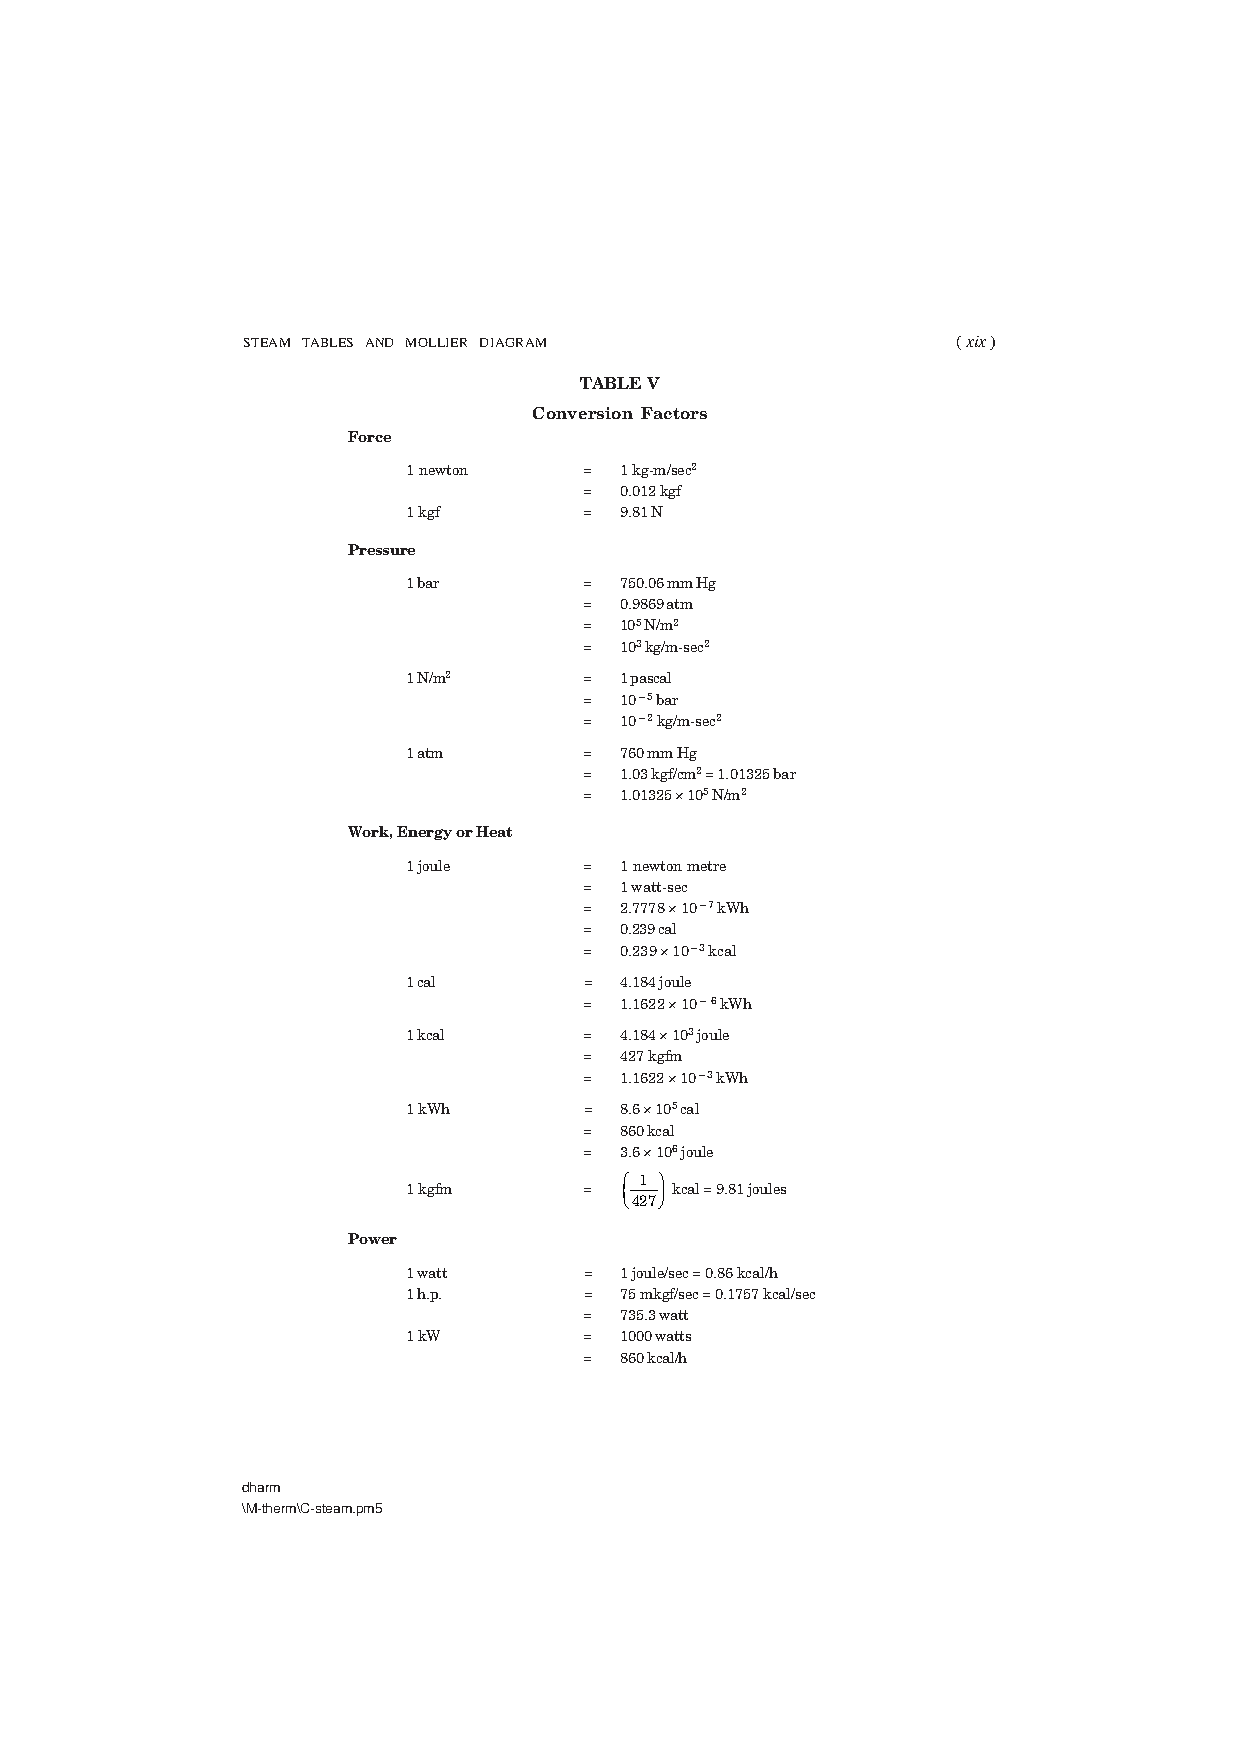
\includepdf[pages=-,fitpaper]{UnitsConversion}
%  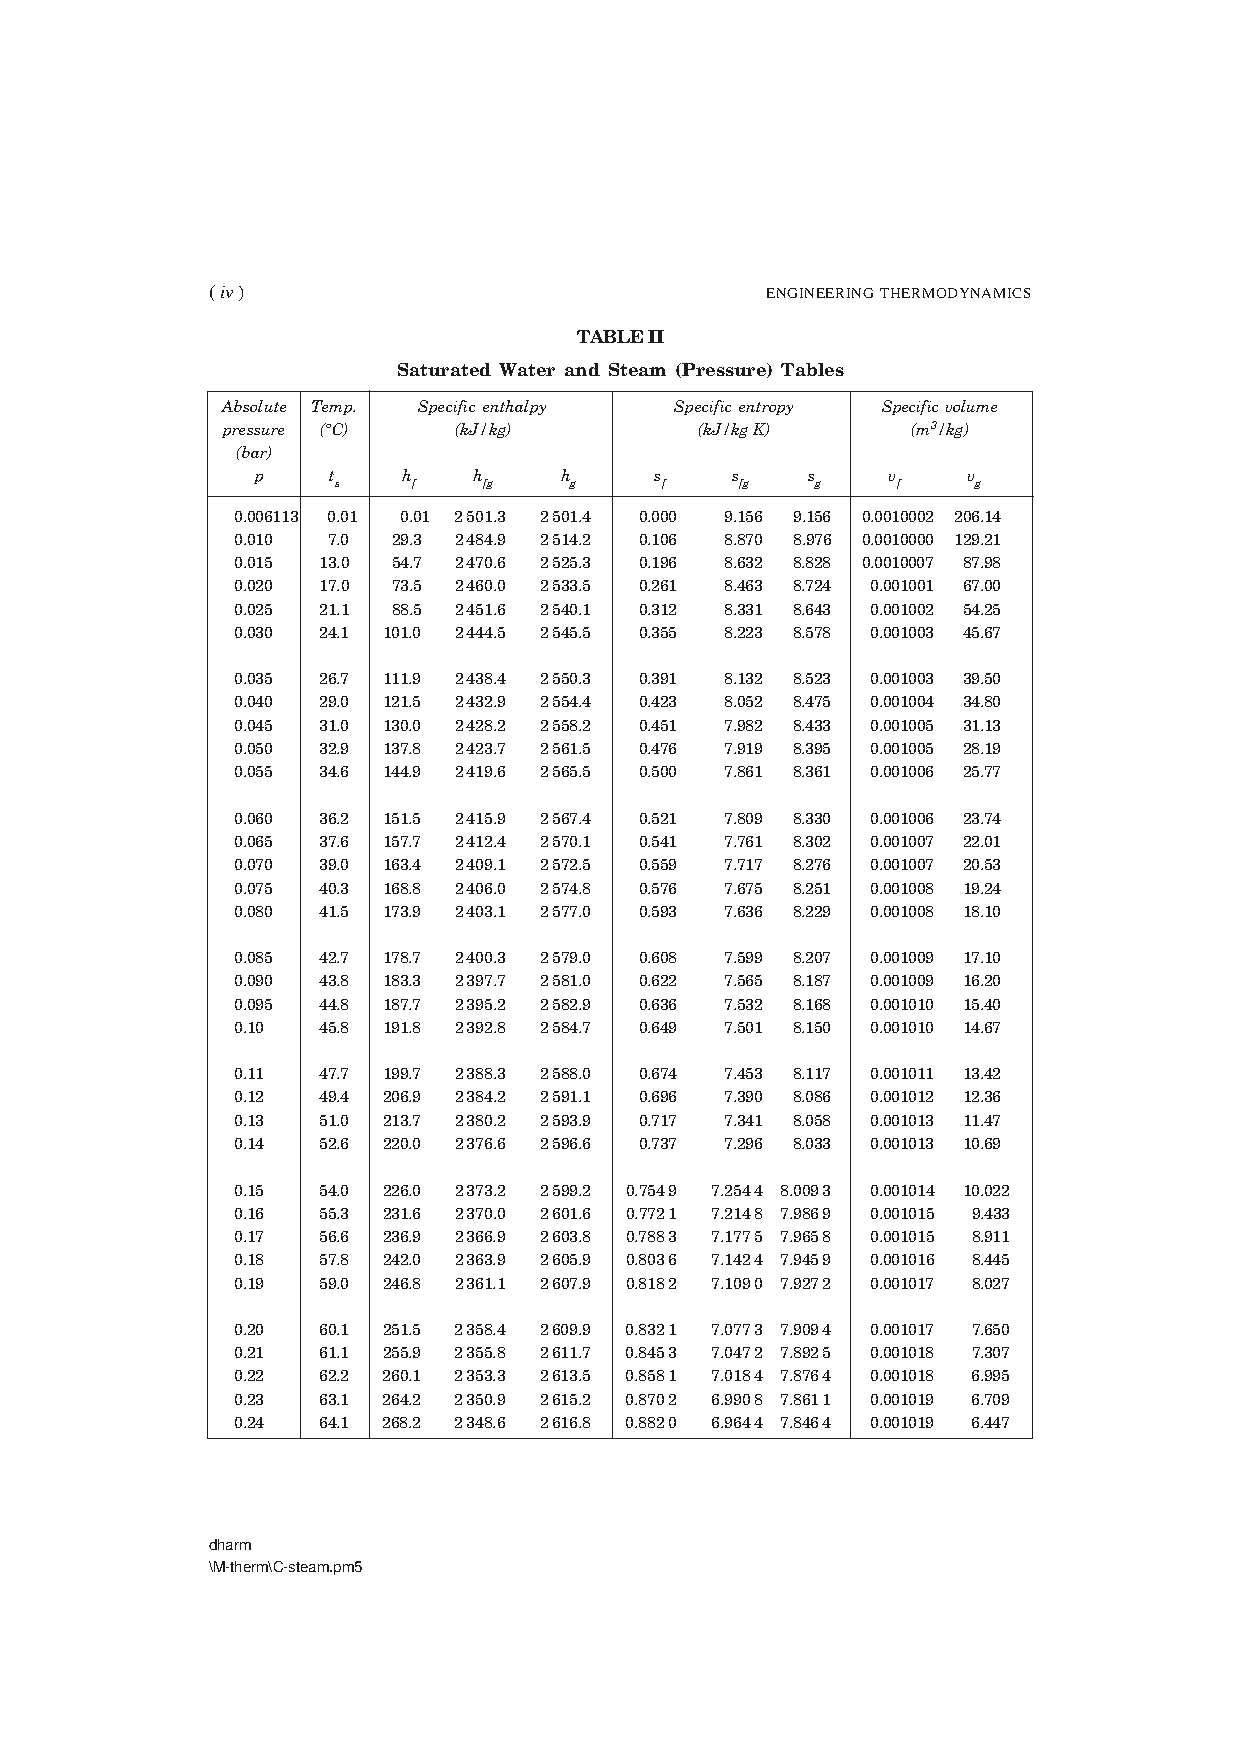
\includepdf[pages=-,fitpaper]{SteamTable_2}
%  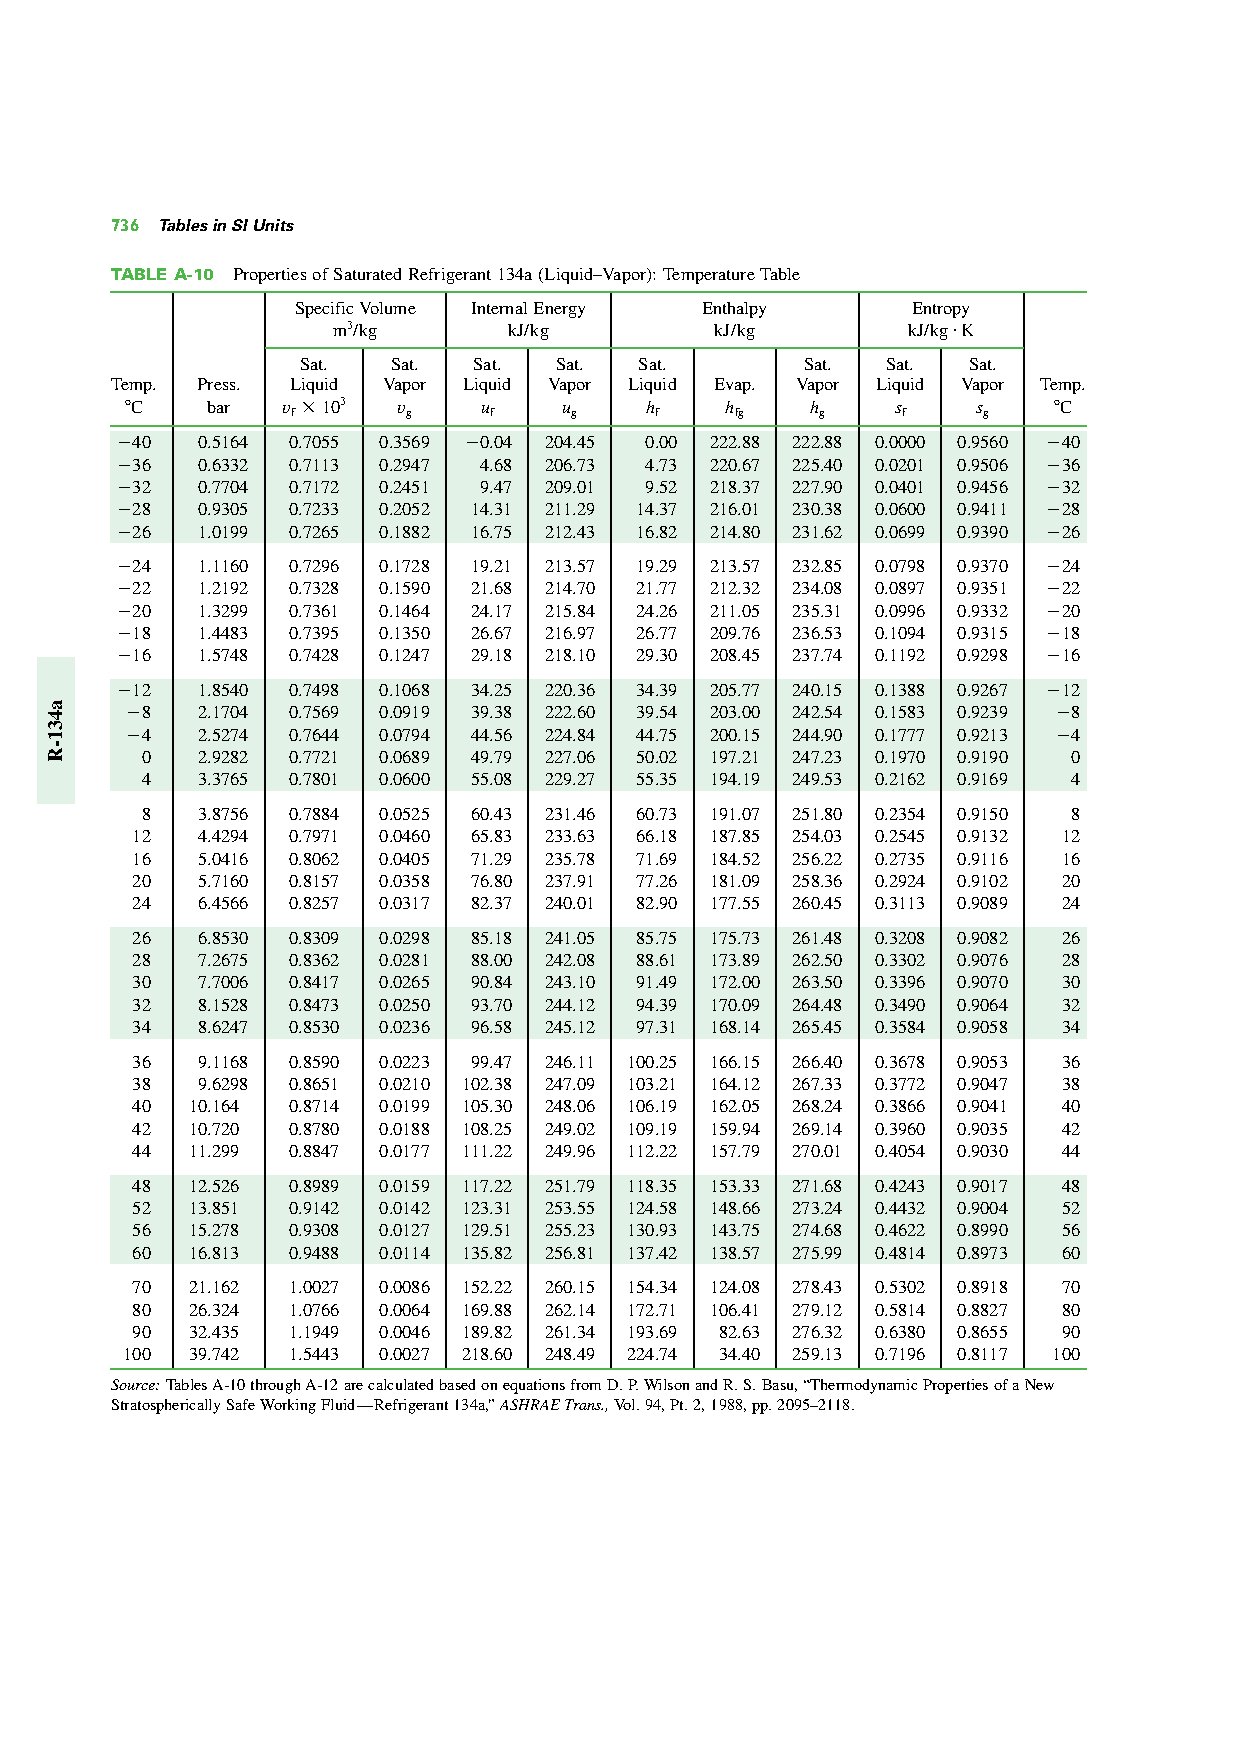
\includepdf[pages=-,fitpaper]{Tables_R134}
%}
%\end{landscape}
%\end{comment}

\end{document}
